\chapter{Lab Maintenance} \label{ch:lab_maintenance}
\section{Pushing Commands and Updates} \label{sec:ssh_push}
\subsection{Remote Commands Background}
In a large environment with hundreds of systems, a method to push commands and updates to them needs to be in place.  This is a separate process from installing and cloning a lab.  For example, all systems in a lab need to be shut down for a planned power outage to the building or some other maintenance.  Without a method to remotely shut them down, a team of techs is needed to go to every system and shut them down cleanly.  This method quickly becomes impractical in labs with hundreds if not thousands of machines.  

Historically, Remote Shell (RSH), part of the rlogin tools, has been used for this purpose.  RSH uses the TCP port 514 to send remote commands to hosts.  It does this by using the username and the source host sending the commands as the authentication mechanism.  So long as this combination is in the authorized hosts ``.rhosts" file, the command will be accepted.  This is done without any form of encryption over a TCP connection.  In an area where the network is heavily secured, this is not necessarily a bad idea and in the past has been used in our labs.  However, it is fairly trivial to spoof an RSH command by impersonating a user and host.  

The telnet protocol can also be used for this purpose.  This protocol requires a username and password to authenticate.  It uses TCP port 23.  Like RSH, it is not encrypted.  While it would be harder to spoof, it is possible to sniff network traffic and gather the authentication credentials.  It is also possible to do a man in the middle attack.  This is less of an issue on switched networks then it was on hubs historically, but the threat of this occurring still exists, especially if the credentials used are the same for all machines.  In addition, scripting a telnet command can be tricky without using a language that can expect a password prompt and act accordingly.

\subsection{Secure Shell Authorized Keys}
As of this writing, the most common protocol used is Secure Shell (SSH).  SSH functions similarly to telnet as far as functionality goes.  However, SSH uses public key exchange to create an encrypted channel.  In addition, it uses host key identification to make sure that the host connected to is who it says it is.  Thus, unless the user disables strict host key checking,\footnote{Strict host key checking is enabled by default on OpenSSH servers.} an SSH session is practically immune to man in the middle attacks and much more difficult to spoof than RSH or telnet methods.   

An SSH session begins by establishing a connection and then exchanging host keys.  SSH authentication comes in either via username/password or via authorized keys.  Username/password prompts function the same as telnet and are thus not very useful for pushing out commands to a lab.

For the purposes of pushing out remote commands, authorized keys are used to prevent the slow process of typing in passwords for every machine pushed to.  Keys come in pairs of public keys and private keys.  Each user can generate a key pair using the SSH-keygen command.  To authenticate with keys instead of passwords, your generated private key should be kept in a ``.SSH/" directory of your user account.  Your matching public key is sent to a remote host which uses it to encrypt traffic to send back to you.  For example, if you push your public key out to root's home directory on a system, you will be able to login as root on that system without a password.  Furthermore, due to the key length, it is much more difficult to brute force a private key than it is a password, and dictionary attacks are practically worthless in this context.  In the CECS labs, we build the master image with the keys and configuration files already in place.  A diagram of how the pushes work can be found in Figure~\ref{fig:sshpush}.

\begin{figure}
  \begin{center}
    \scalebox{0.7}{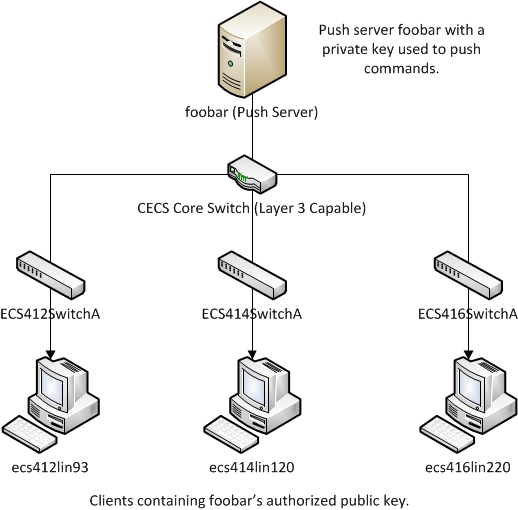
\includegraphics{../figures/sshpush.png}}
  \end{center}
  \caption{SSH remote command push.}
  \label{fig:sshpush}
\
\vskip1pt
\
\vskip1pt
\
\end{figure}


Because a password prompt never occurs, SSH can be used to run a command immediately after authentication.  With the use of semicolons and other special shell characters, multiple commands can be run.  Hypothetically, a command to download a script from a webserver can be followed by the command to run that script.  However, each system touched must have their public key accepted by the push server at least once to prevent prompts from occurring during automation.  For clones, it is useful to have all the clones use the same key.  And for subsequent clones, the previous key may be used to prevent SSH from failing due to a key identification mismatch.  This should not be done in highly secure environments though, as it circumvents protection against man in the middle attacks.  

\subsection{Push Script}
Thus, a relatively short script can be written to send commands to all participating servers.  In its simplest form, all this script does is loop through a list of hosts and execute the SSH command on each host.  In some shells, the loop may malfunction if SSH is not run in batch mode to prevent stdin, so care must be taken to remember that argument if using such a Unix shell.  

A more advanced script would fork each SSH command to the background to run commands on hosts in parallel.  This has the potential to overload the push server,\footnote{The push server is most likely to be a fairly old machine.} so adding a delay after so many forked commands would help if the CPU is being taxed too much.  A fair amount of CPU cycles are used to negotiate the key exchange and encrypt the traffic.  The other issues that may occur are hosts that hang the SSH session.  This will cause the SSH command process to hang until killed.  Sometimes it can only be killed with signal 9.  If hosts do not seem to be doing this often, it may be fine to overlook and fix them manually after the script is run.\footnote{We log the malfunctioning systems and investigate them later.}  To remedy failed SSH sessions, at the end of the script, we force the script to sleep for a reasonable amount of time then kill all SSH sessions with the ``killall" command.  

